\documentclass{scrartcl}
\usepackage[latin1]{inputenc}
\usepackage[T1]{fontenc}
\usepackage{url}
\usepackage{graphicx}
\usepackage{ae}
\usepackage{hyperref}


\newcommand{\theTitle}{Documentation for Law Leecher 1.2}
\newcommand{\theAuthor}{Tobias Vogel}

\hypersetup{
draft=false,
pdftitle={\theTitle},
pdfcreator={\theAuthor},
pdfauthor={\theAuthor},
pdfsubject={\theTitle},
pdfproducer={\theAuthor},
  linkcolor=black,        % color of internal links
  citecolor=black,        % color of links to bibliography
  filecolor=black,           % color of file links
  urlcolor=black,          % color of external links
  colorlinks=true
}

\begin{document}

\title{\theTitle}
\author{\theAuthor\\\url{tobias@vogel.name}}
\date{\today}

\maketitle

\begin{abstract}
This documentation comprises goal, installation instruction, usage manual, implementation details for \textit{Law Leecher}, a tool for retrieving data from the PreLex database.

\textit{Law Leecher} is published under the 3-clause BSD license.\footnote{\url{http://en.wikipedia.org/wiki/BSD_licenses\#Terms}}
\end{abstract}


\tableofcontents


\section{Preface}
The decision-making process between institutions in the European Union is documented and freely available under \url{http://ec.europa.eu/prelex/apcnet.cfm?CL=en}. This web page contains about 30,000 laws\footnote{In this document, they are called laws, even if they did not evolve to a adopted law.} by October 2009. To drive statistical analysis on this data, it has to be extraced from this web database, first.

To retrieve this structured data, a tool coined \textit{Law Leecher} has been developed. This document fulfills three purposes:

\begin{itemize}
\item It shows, which \textit{information} is extracted.
\item It is a \textit{user manual}.
\item It serves as \textit{source code documentation}.
\end{itemize}



\section{Extracted Information}
The details of each law are contained on each law's web page. Figure~\ref{fig:screenshot} shows one of these pages and the pieces of information which are relevant for the crawling. It is annotated with red and black rectangles. The web page always contains some meta information on top, a greenish area below, and finally a number of directly piled up tables which describe the progress of the discussion about the law as a timeline. Each of these tables contains one row with a date stamp and a title and optionally another row with key value pairs. Generally, all HTML markup is removed from the extracted values, e.g., hyperlinks, line breaks, or text formatting and only plain text is saved.

\label{sec:numberingschema}
\begin{description}
\item[Rectangle A] contains information which are retrieved as-is and saved under the name ``bluebox.UpperLeftIdentifier''.
\item[Rectangle B] contains information which are retrieved as-is and saved under the name ``bluebox.UpperCenterIdentifier''.
\item[Rectangle C] contains information which are retrieved as-is and saved under the name ``bluebox.ShortDescription''.
\item[Rectangle D] is characterized by a green background color. It always contains four key value pairs. The keys, which are on green background, are ``Fields of activity'', ``Legal basis'', ``Procedures'', and ``Type of file''. Values are on gray background, some of the laws do not possess a value, others contain line breaks, colons, etc. Values are always transformed to simple strings with all HTML markup removed. The name under which the information is saved is ``greenbox.FieldsOfActivity'', ``greenbox.LegalBasis'', ``greenbox.Procedures'', and ``greenbox.TypeOfFile''.
\item[Rectangle E] is the first table. All key value pairs are read out, for example ``firstbox.Responsible'' or ``firstbox.LegalBasis''. Values for the ``Documents'' key are split and joined with ``, ''.
\item[Rectangle F] is the last table. It contains several key value pairs, but only the values of ``Documents'', ``Procedures'', ``Type of file'', and ``NUMERO CELEX'' are taken as ``lastbox.Documents'', ``lastbox.Procedures'', ``lastBox.TypeOfFile'', and ``lastbox.NumeroCelex''.
\item[Black rectangles] are used differently. As mentioned above, each table consists of a header row which contains a date stamp and a title, and optionally a second row with some key value pairs. These tables are to be read out while grabbing each table's date stamp, the title and---if existing---the value of the key named ``Decision'' or ``Decision mode''. The title is not saved explicitly. Instead, it serves as the prefix. In the figure's first table, which is ``firstbox'' at the same time, this would be ``Adoption by Commission'' with the suffix ``date'' and the value ``01-10-2004'' and the suffix ``decision'' with the value ``Written procedure''. The difference between ``Decision'' and ``Decision mode'' is irrelevant, so that it is always named ``decision''. However, the prefixes are not necessarily unique within one law. That is why they are extended by three-digit numbers, starting with ``001'' for each title, even if this specific title just occurs once in this law. They are numbered from top to bottom. In the figure, this rule creates the following keys: ``Adoption by Commission001.date'' and ``Adoption by Commission.decision''.
\item[Further information] are the law's type ``Type'' and the law's id (``ID''). The id is taken from the HTTP request, it does not appear on the page. The type can be derived from ``bluebox.UpperCenterIdentifier''. It is the abbreviation after the second slash and can have the values ``AVC'', ``COD'', ``SYN'', or ''CNS''. If the type is different or not stated in this area, it is put into the set of extracted data but without a value.
\end{description}

\begin{figure}[ht]
\begin{center}
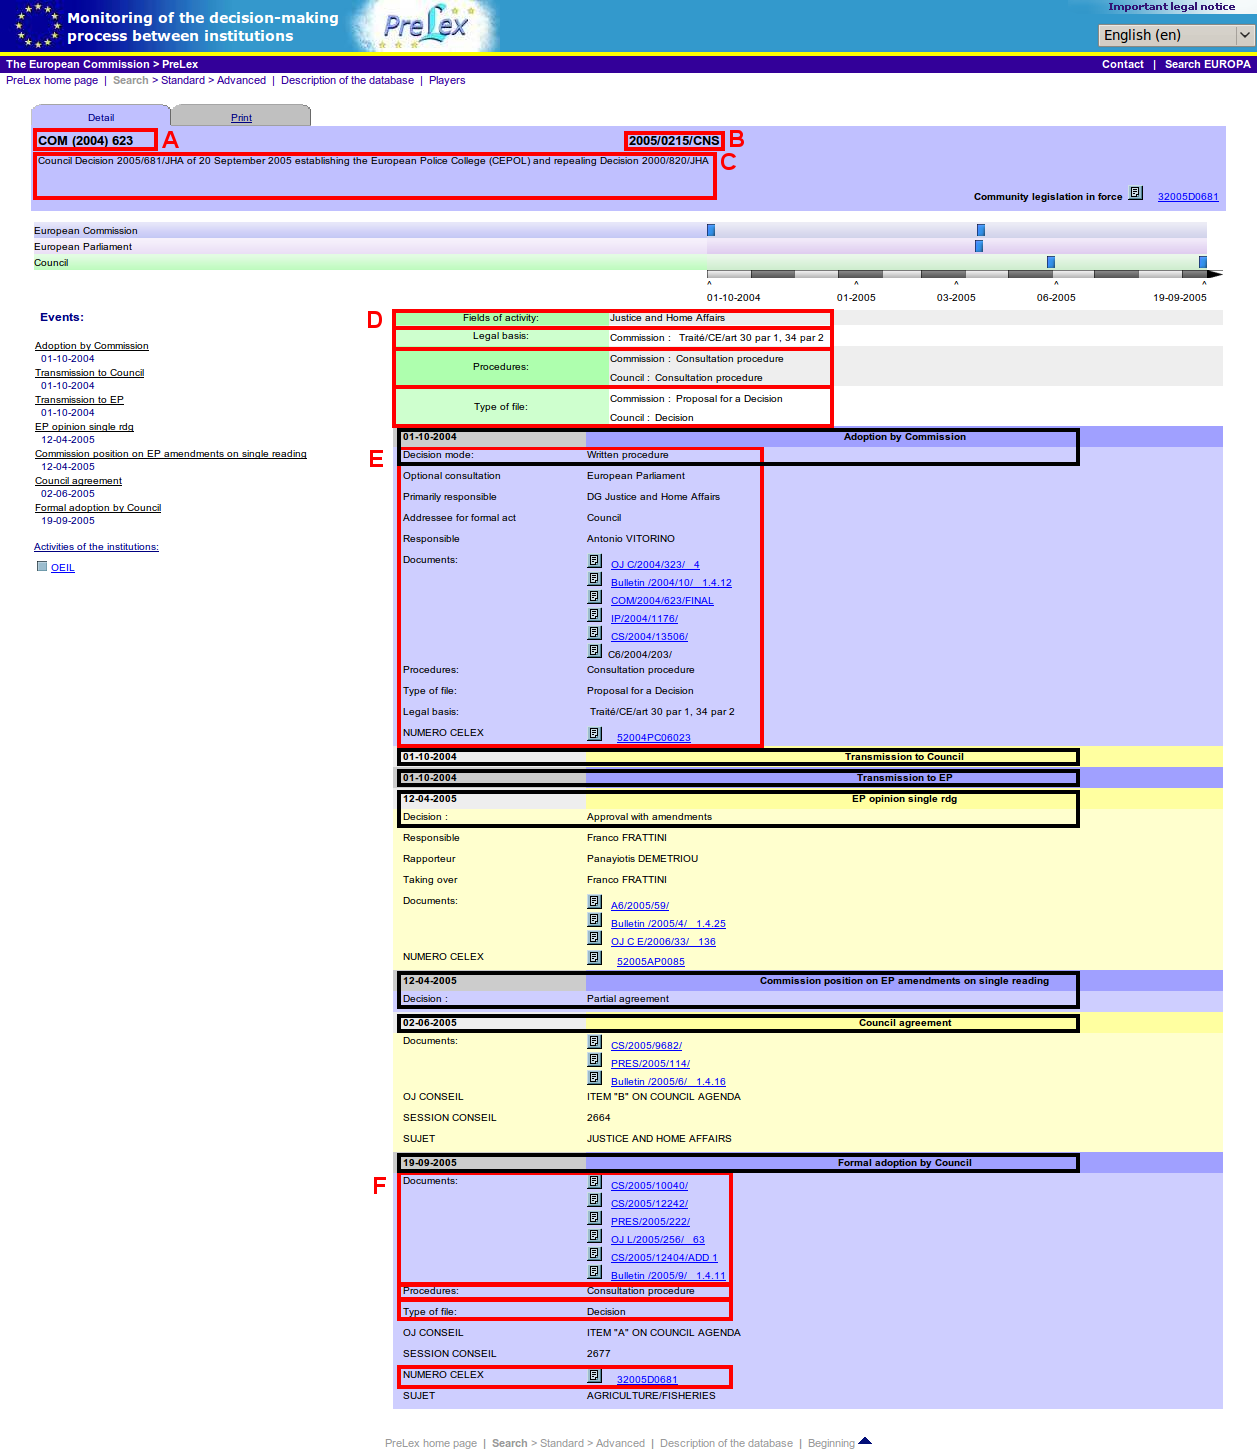
\includegraphics[width = \textwidth]{prelex.png}
\caption{Website content of law 191763 with annotated relevant sections.}
\label{fig:screenshot}
\end{center}
\end{figure}

\clearpage

If the list of tables just contains one table, this is not handled differently and thus, the values are extracted twice.
The full retrieved record for this law would be as follows (noted in a JSON-like notation):

\begin{verbatim}
{
  ID = 191763,
  Type = CNS,
  bluebox = {
    UpperLeftIdentifier = COM (2004) 623,
    UpperCenterIdentifier = 2005/0215/CNS,
    ShortDescription = Council Decision 2005/681/JHA of 20 September 2005 establishing the European Police College (CEPOL) and repealing Decision 2000/820/JHA
  },
  greenbox = {
    FieldsOfActivity = Justice and Home Affairs,
    LegalBasis = Commission : Traité/CE/art 30 par 1, 34 par 2,
    Procedures = Commission :Consultation procedure Council :Consultation procedure,
    TypeOfFile = Commission :Proposal for a Decision Council :Decision
  },
  lastbox = {
    Documents = CS/2005/10040/, CS/2005/12242/, PRES/2005/222/, OJ L/2005/256/ 63, CS/2005/12404/ADD 1, Bulletin /2005/9/ 1.4.11,
    Procedures = Consultation procedure,
    TypeOfFile = Decision,
    NumeroCelex = null
  },
  firstbox = {
    Addressee for formal act = Council,
    Decision mode: = Written procedure,
    Documents: = OJ C/2004/323/ 4, Bulletin /2004/10/ 1.4.12, COM/2004/623/FINAL, IP/2004/1176/, CS/2004/13506/, C6/2004/203/,
    Legal basis: = Traité/CE/art 30 par 1, 34 par 2,
    NUMERO CELEX = 52004PC06023,
    Optional consultation = European Parliament,
    Primarily responsible = DG Justice and Home Affairs,
    Procedures: = Consultation procedure,
    Responsible = Antonio VITORINO,
    Type of file: = Proposal for a Decision
  },
  timeline = {
    Adoption by Commission001 = {
      date = 01.10.04,
      decision = Written procedure
    },
    Commission position on EP amendments on single reading001 = {
      date = 12.04.05,
      decision = Partial agreement
    },
    Council agreement001 = {
      date = 02.06.05,
      decision = null
    },
    EP opinion single rdg001 = {
      date = 12.04.05,
      decision = Approval with amendments
    },
    Formal adoption by Council001 = {
      date = 19.09.05,
      decision = null
    },
    Transmission to Council001 = {
      date = 01.10.04,
      decision = null,
    },
    Transmission to EP001 = {
      date = 01.10.04,
      decision = null
    }
  }
}
\end{verbatim}


%\clearpage

\section{Installation and Usage}
\subsection{Installation}
Follow these steps to install Law Leecher on Windows (tested on Windows~XP).
\begin{enumerate}
\item Download the One-Click Installer from \url{http://rubyinstaller.org/} to install Ruby. Install it under the proposed directory, \texttt{c:\textbackslash ruby}. Accept the wizard's proposals for all other options, but activate the European Keyboard option.

\item Second, install the toolkit which provides the GUI. It's named \textit{GTK+}. Download it from \url{http://prdownloads.sourceforge.net/ruby-gnome2/ruby-gnome2-0.16.0-1-i386-mswin32.exe?download}. When following the wizard, correct the path of the Ruby installation in case that there are special characters at the end of the path string. 
\end{enumerate}

In case of problems, follow the instructions on \url{http://ruby-gnome2.sourceforge.jp/hiki.cgi?Install+Guide+for+Windows}.

\subsection{Usage}
Law Leecher provides both, an easy-to-use GUI in German language and a powerful command line interface.

\subsubsection{Graphical User Interface}
\begin{figure}[ht]
\begin{center}
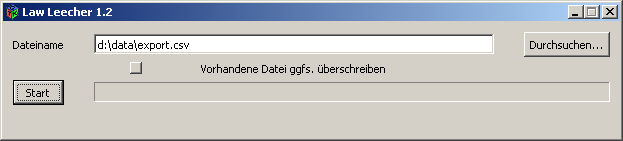
\includegraphics[width = \textwidth]{GUI.png}
\caption{The graphical user interface of the program.}
\label{fig:guiwindow}
\end{center}
\end{figure}

Start the program by invoking \texttt{main.rb}. The window as depicted in Figure~\ref{fig:guiwindow} should become visible. In the input area, type in the path and the file name of the output file. You can use the button on the right to select it by browsing over the file system. Check the check box under the input to overwrite a possibly existing file. You will get a warning message in advance of starting the process, if a file exists there and you didn't check the check box. Press the start button to start the process. You can only abort it by closing the window which might take a while. Law Leecher takes about 8 minutes to retrieve 1000 laws on an average DSL connection.

\subsubsection{Command line client}
Law Leecher offeres a command line client for batch processing. It can be called via \texttt{ruby main.rb ---nogui} and it has the following optional parameters. The notation is \texttt{---parameter=value} except for parameters which are simple flags.
\begin{description}
\item[\texttt{---startyear}] Law Leecher crawls laws from this start year to the current year. The default start year is 1969.
\item[\texttt{---numberofthreads}] Law Leecher is multi-threaded (c.f. Section~\ref{sec:threading}). By default, it uses 8 worker threads to retrieve and parse law web pages.
\item[\texttt{---filename}] The default output file is called ``export.csv`` and will be placed directly in the directory where main.rb is located. You can change it here.
\item[\texttt{---overwriteexistingfile}] Use this option to allow Law Leecher to overwrite an existing output file.
\end{description}

When you call it without the \texttt{---nogui}, the GUI will be started and all command line parameters will be ignored.



\section{Implementation Details}
This section will describe the architecture of the program. It will not got into too much detail, since the code is well-documented. Instead, some important aspects are emphasized and the main functionality of the existing classes are explained.

\subsection{Architecture}
Figure~\ref{Architecture} shows the architecture of the program.

\begin{figure}[ht]
\begin{center}
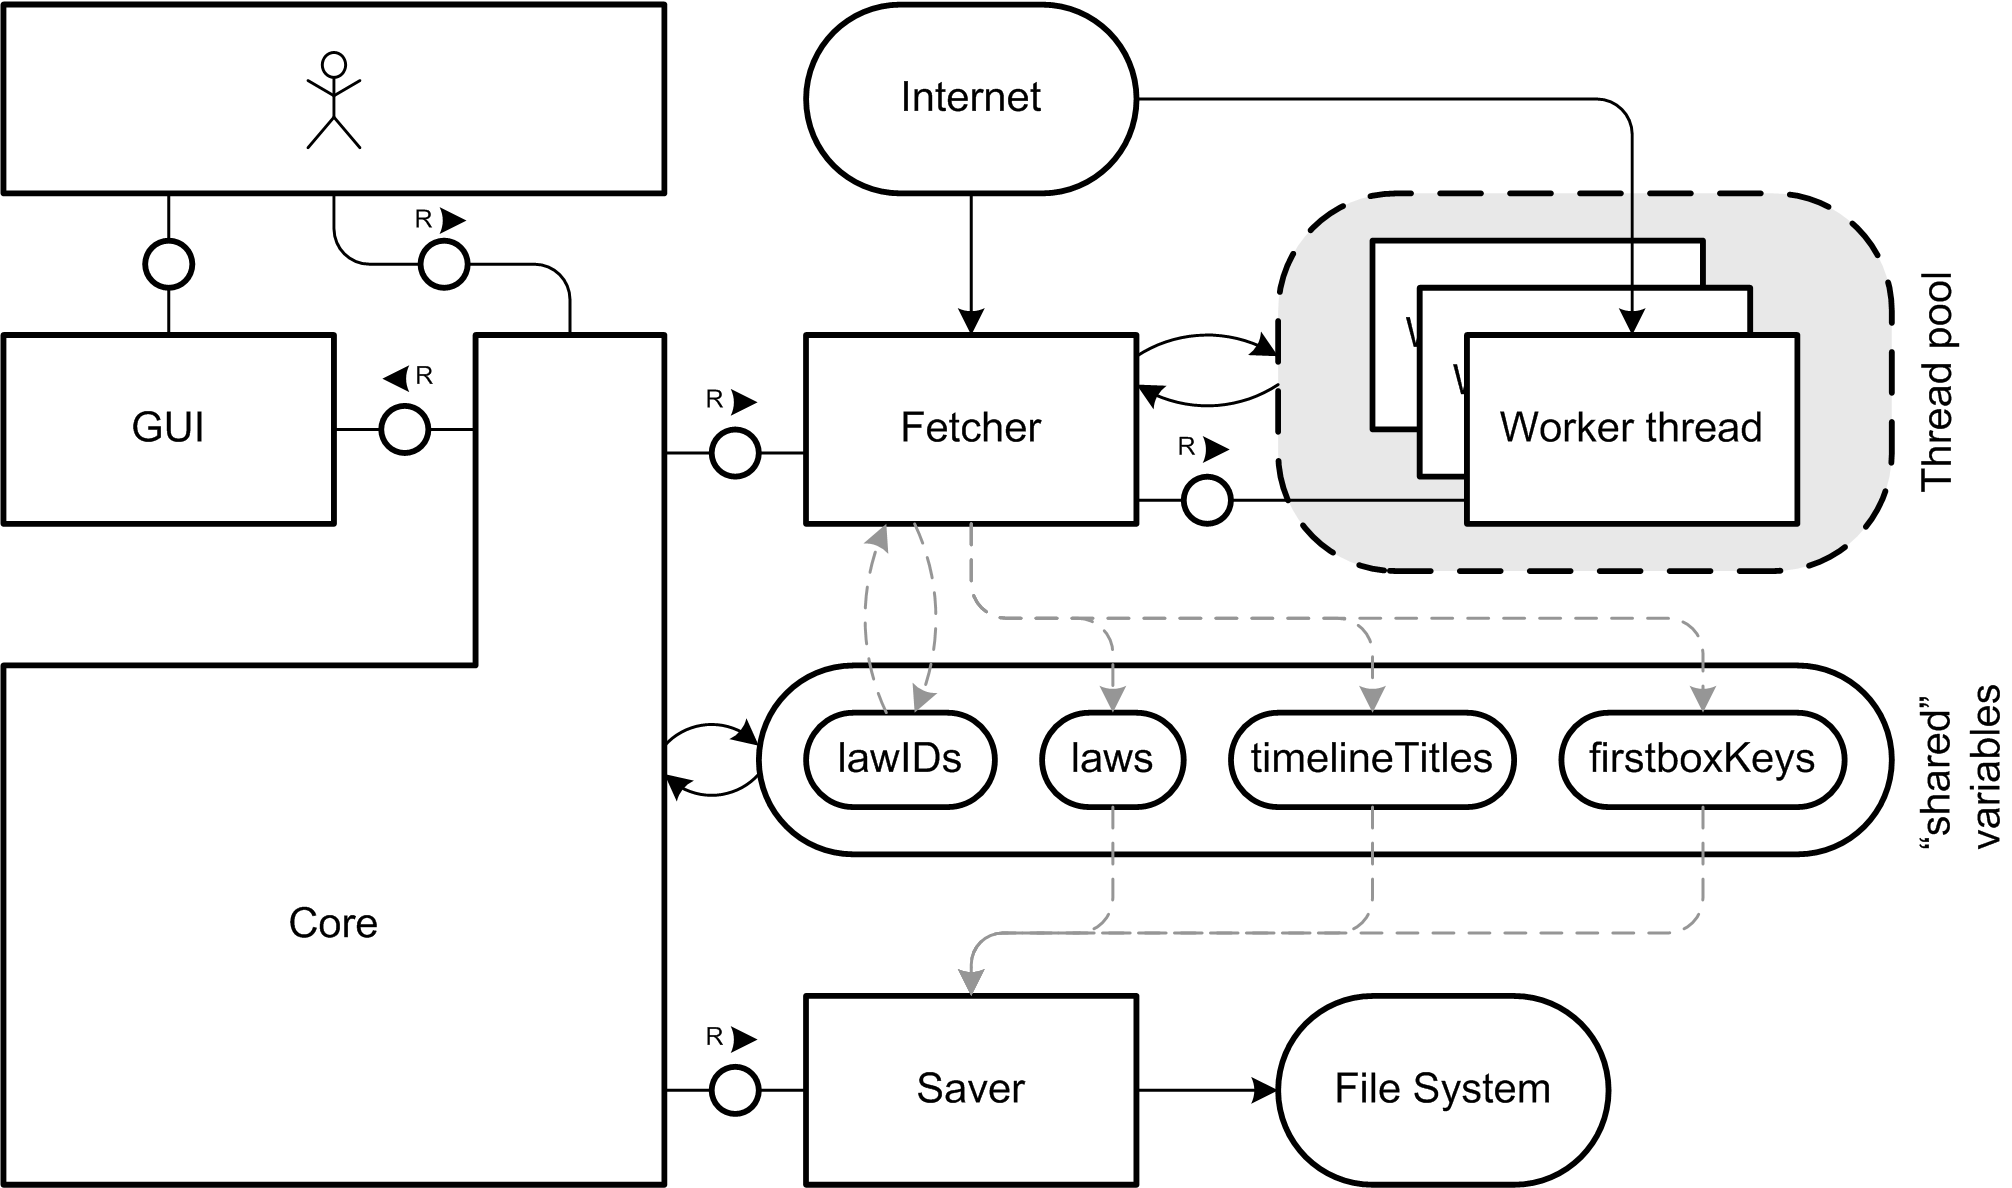
\includegraphics[width = \textwidth]{Architecture.png}
\caption{The basic architecture of the program}
\label{Architecture}
\end{center}
\end{figure}

The user starts the program (\textit{Core}) which controls all components and additionally enables the user to communicate with the program via the \textit{GUI}. The program's task is to retrieve laws from the Internet and to save them on the disk. This is done by the \textit{Fetcher} and the \textit{Saver}.

In the beginning, the Core starts the Fetcher to fetch all IDs of the laws to retrieve. The IDs are saved in the \texttt{lawIDs} variable. Next, the Core calls the Fetcher again to retrieve and parse the single web pages. The result is written into the \texttt{laws} variable. To speed up the retrieval process, the Fetcher uses several threads for retrieval and scraping. Finally, the Saver writes all the laws to the file system.

Because the laws have partially different keys, e.g., depending from the different number of tables in them, all keys from all laws are taken to create a huge, sparse table, where each column is at least populated with one value of one law, but many columns mostly stay empty. To get all the column headers, \texttt{timelineTitles} and \texttt{firstboxKeys} are filled by the Fetcher, where the keys are sorted and rewritten concerning the numbering schema described in Section~\ref{sec:numberingschema}.

The depicted 4 variables can only be written by the Core. To illustrate, which component conceptually writes on/reads from them, gray, dashed arrows are used.

Each agent is implemented within a class of the same name. The starting method is located within \texttt{main.rb}, which is no class. GUI and Core are singletons.

\subsection{Implementation Details}
The code is entirely written in Ruby and in English language. Only the GUI output is German.

\subsubsection{Threading}
\label{sec:threading}
The fetcher holds a list of IDs for laws which still are to process. When there are less than the specified number of threads running, it removes the first ID of this list and starts a new thread (a \textit{Parser Thread}) processing this ID (retrieval and parsing). Most of the time, all threads are busy. Then the thread iterates over a list of running threads to check, whether there is a finished thread. If a thread has finished, its return value (a big hash array) is added to the result list. There is no Mutex mechanism that allows threads to individually save information into a central variable.

\subsubsection{GUI Callbacks}
The system is designed to work with and without a GUI. To provide status information to the GUI, callbacks are used. The Core contains a method coined \texttt{callback} which receives textual information. This information is printed to the console. If the program runs in GUI mode, this information is also forwarded to the \texttt{updateWidgets} method of the GUI class. Information which is not intended to be sent to the GUI is simply printed with a ``puts''.

\subsubsection{Regular Expressions}
Ruby 1.8 does not support variable-length lookbehinds. To overcome this deficit, the ParserThread class has the method \texttt{parseSimple} which takes two patterns and the string to apply the Regular Expressions on. The second pattern should start with \texttt{.*} to match the desired substring. Afterwards, an arbitrary lookahead pattern can be contained. The first pattern contains the desired lookbehind without the \texttt{(?<=...)} specification.

The method first extracts the concatenation of the first and the second pattern from the string and then replaces the first pattern with an empty string in the intermediate result. 

\subsubsection{Unicode}
The text on the website is provided in Unicode. It has to be translated into ANSI (Latin-1), because Excel interprets CSV files in such a way. This translation has been outsourced in the Saver's \texttt{convertUTF8ToANSI()} method which simply returns the converted string.

\subsubsection{GUI Implementation}
The GUI contains a description of all widgets in the window. It's programmed with GTK2. It also connects the widgets with the appropriate functions in the program.

The GUI is held responsive by implementing a cooperative multitasking. From time to time (more exact: at the beginning of each law processing via the \texttt{informUser()} method), the method \texttt{updateWidgets()} is called. The provided hash contains a bunch of information to update. That may be the progress bar or the status message. Afterward, a pending events handling loop is executed, allowing to move the window and to redraw the recently edited text.

\subsubsection{Default Values}
The Configuration class contains global variables and their getters and setters which are used throughout the program.

\subsection{Benchmark}
To find out the optimal number of worker threads and to evaluate the usefulness of the usage of threads, a benchmark was driven. 1500 laws were retrieved with 1 to 24 threads, where each run was repeated twice to eliminate the bias. Figure~\ref{fig:benchmark} shows the results.

\begin{figure}[ht]
\begin{center}
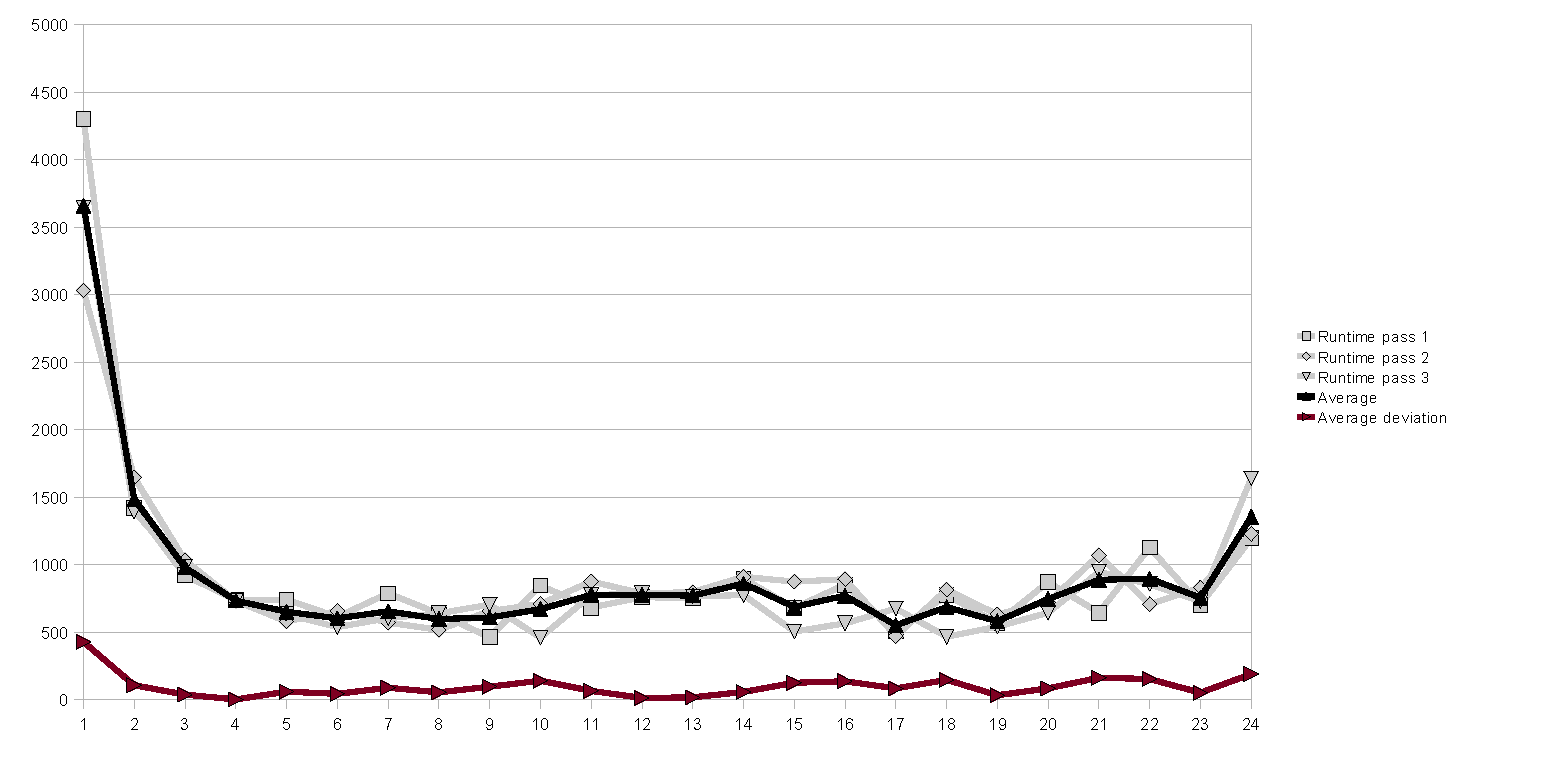
\includegraphics[width = \textwidth]{benchmark}
\caption{Benchmark for the average runtime in seconds (black) among three runs (gray) for 1500 laws. The x axis shows the number of threads employed. The brown line depicts the average deviation from the average. With more than 4 threads there is no substantial decrease in runtime.}
\label{fig:benchmark}
\end{center}
\end{figure}

\subsection{Pitfalls}
\subsubsection{Interpreter}
The default ruby interpreter is able to run the full program, currently. However, the JRuby interpreter runs into memory problems with the current implementation. These problems appreared on a 2 GHz dual-core, 4 GB RAM, Ubuntu 9.04 64 Bit machine with the JRuby interpreter set to \texttt{-Xms32m, -Xmx2048m -XX:-UseGCIOverheadLimit}.
\end{document}
